\documentclass[12pt,t]{beamer}
\usepackage[brazil]{babel}
\usepackage[utf8x]{inputenc}
\usepackage{beamerthemeboadilla}
\usepackage[alf]{abntex2cite}	
\usepackage{tabulary}
\usepackage{tabularx} 
\usepackage{booktabs}
\usepackage{multirow}
\usepackage{caption}
\usepackage{listings}
\usepackage{graphicx}
\usepackage{epstopdf}
\usepackage{etoolbox}
\usepackage{mathabx}
\usepackage{url}
\usepackage{listings}

\usepackage[htt]{hyphenat}
\usepackage{etoolbox}
\usepackage[abs]{overpic}

\usepackage{tikz}
\usetikzlibrary{shapes.geometric, arrows}

\newcommand\eqdef{\mathrel{\overset{\makebox[0pt]{\mbox{\normalfont\tiny\sffamily def}}}{=}}}

\defbeamertemplate{description item}{align left}{\insertdescriptionitem\hfill}

\institute{POO 2015\\IME -- USP}
\author{Bruno Sofiato\\Vinicius Nascimento Silva}

\title{Reflexão computacional e meta-objetos}

\makeatletter
\patchcmd{\beamer@sectionintoc}
{\vfill}
{\vskip\itemsep}
{}
{}
\makeatother  
%\usepackage{default}

\AtBeginSection[]{
	\begin{frame}[c]{ }
		\centering
		\begin{beamercolorbox}[sep=8pt,center,shadow=true,rounded=true]{title}
			\huge\insertsectionhead\par%
		\end{beamercolorbox}
	\end{frame}
}


\begin{document}
\abovedisplayskip=0pt
\abovedisplayshortskip=0pt
\belowdisplayskip=0pt
\belowdisplayshortskip=0pt	
 \frame{\titlepage}
 \begin{frame}{Agenda}
	\tableofcontents
 \end{frame}
 \section{Introdução}
 \begin{frame}{XXX}
 	Colocar algumas estatísticas, não sei muito bem o que colocar aqui.
 	Colocar que o foco sera linguagens orientadas à objetos baseadas em classe.
 \end{frame}
 \section{Meta-modelo}
	 \begin{frame}{Meta-}
	 	\begin{block}{Etimologia}
	 		O prefixo meta- remete ao grego \alert{COLOCAR}, que significa \emph{além} ou \emph{depois}.
	 	\end{block}
	 	\begin{block}{Significado}
	 		Geralmente é usado para representar um conceito que é uma abstração de outro.
	 	\end{block}
	 	\begin{exampleblock}{Exemplos}
	 		\begin{description}[Metalinguagem]
	 			\item [Metafísica]  		\alert{Colocar um texto legal}
	 			\item [Metalinguagem] São linguagens utilizadas para definição de outras linguagens:
	 			\begin{itemize}
	 				\item EBNF 
	 				\item XML (schema)
	 			\end{itemize}
	 		\end{description}
	 	\end{exampleblock}
	 	\end{frame}
	 	\begin{frame}{Metamodelos}
	 		\begin{block}{Definição}
	 			Informalmente é um modelo de um modelo.
	 		\end{block}
	 		\begin{block}{Usos}
	 			Normalmente, são utilizados em ferramentas que oferecem suporte à criação de modelos. Entre elas, ferramentas de CAD, CAE e CASE.
	 		\end{block}
	 		\begin{exampleblock}{Exemplos}
	 			\begin{description}[Datawarehousing]
	 			\item [Construção Civil] \emph{Building Information Model} (BIM);
	 			\item [Datawarehousing]		
	 		\emph{Common Warehouse MetaModel} (CWM);
	 			\item [Matemática] Teoria das Categorias;
	 			\item [Programas OO] \emph{Unified Modeling Language} (UML).
	 		\end{description}
		\end{exampleblock}
	 \end{frame}
	 \begin{frame}{MOF -- Meta-object Facility}
	 	\begin{block}{Características}
	 		\begin{itemize}
	 			\item Definida pela OMG (Object Management Group) para a modelagem de metadados (versão atual -- 2.4.2);
	 			\item Define quatro camadas (do nível três ao zero).	
	 		\end{itemize}
	 	\end{block}	 
	 	\begin{block}{ }
	 		\alert{FIGURA -- adaptar da pagina MOF da wikipedia}
	 		%\url{http://en.wikipedia.org/wiki/Meta-Object_Facility#/media/File:M0-m3.png}
	 	\end{block}
	 \end{frame}
	 \begin{frame}{Meta-modelo UML}
	 	\begin{block}{Características}
	 		\begin{itemize}
	 			\item Mantido pela OMG, define a estrutura e a semântica dos construtos da UML (versão atual -- 2.4.2);
	 			\item Incluso na 2a camada MOF;
	 			\item Descrito em dois manuais complementares:
	 			\begin{description}[Superestrutura]
	 				\item [Infraestrutura] \alert{Escrever o que é}
	 				\item [Superestrutura] \alert{Escrever o que é}
	 			\end{description}
	 		\end{itemize}
	 	\end{block}
	\end{frame}
	 \begin{frame}{Metamodelo UML -- Trecho}
	 		\alert{FIGURA (trecho do meta-modelo)}
	 \end{frame}
	% \begin{frame}[c]{ }
	%	\centering
	%	\LARGE E se esse modelo estivesse disponível em tempo de execução ?
	% \end{frame}
 \section{Programação Reflexiva}
	 \begin{frame}{O que é reflexão}
	 	\begin{block}{Definição}
	 		\emph{''It's all about building your language out of first-class, dynamic object that you can look at and change at runtime''}
	 		\begin{flushright}
	 			Brian Foote
	 	\end{flushright} 	 		
	 	\end{block}
	 	\begin{block}{História}
	 		\begin{description}[9999]
	 			\item[1982] Definição por \citeonline{smith1982reflection} das características de sistemas ditos reflexivos;
	 			\item[1983] Smalltalk-80 incorpora a noção classes sendo objetos -- podendo assim responder à mensagens;
	 			\item[1984] \citeonline{friedman1984reification} descrevem um mecanismo que permite a criação de sistemas reflexivos;
	 			\item[1991] \citeonline{kiczales1991art} escreve o livro \emph{The Art of Metaobject Protocol}.
	 		\end{description}
	 	\end{block}	
	 \end{frame}
	 \begin{frame}{Procedural reflection in programming languages \cite{smith1982reflection}}
	 	\begin{block}{Descrição}
	 		Na tese de doutorado de Brian Cantwell Smith (\emph{Procedural reflection in programming languages}), são definidas três caraterísticas básicas necessárias em sistemas reflexivos. 
	 	\end{block}
	 	\begin{block}{Características -- Sistemas Reflexivos}
	 	  \begin{enumerate}
	 	  	\item Um sistema deve ter uma representação de si mesmo;
	 	  	\item Deve haver uma conexão causal entre um sistema e sua representação;
	 	  	\item Devem existir mecanismos com os quais um programa pode manipular sua representação. 
	 	  \end{enumerate}
	 	\end{block}
	 \end{frame}
	 \begin{frame}{Reification -- Reflection without Metaphysics  \cite{friedman1984reification}}
	 	\begin{block}{ }
	 		\alert{Colocar figura}
	 	\end{block}
	 	\begin{block}{Operações}
	 	\begin{description}[reificação]
	 				\item [reificação] Transforma o programa em execução em uma representação a ele disponível;
	 				\item [reflexão] Reflete, em um programa em execução, as modificações realizadas na sua representação.
	 			\end{description}
	 	\end{block}
	 	
	 \end{frame}	  	 
  	 \begin{frame}{The Art of Metaobject Protocol \cite{kiczales1991art}}
  	 	\begin{block}{Descrição}
  	 		Descreve a implementação do protocolo de metaobjetos do CLOS (Common Lisp Object System).
  	 	\end{block}
  	 	\begin{block}{Protocolo de Metaobjetos}
  	 		\begin{itemize}
  	 			\item É a interface para acesso aos metaobjetos de um sistema (semelhante ao conceito de protocolo de Smalltalk);
  	 			\item Dependente de linguagem ($\neq$ Metamodelo UML);  
  	 			\item Suas operações podem ser agrupadas em dois grupos:
  	 			\begin{description}[Introspecção]
  	 				\item [Introspecção] Examinam a estrutura e estado do programa;
  	 				\item [Intercessão] Realizam mudanças estruturais e comportamentais no programa.
  	 			\end{description}
  	 		\end{itemize}
  	 	\end{block} 
  	 \end{frame}	
 	 \begin{frame}{Introspecção}
 	 	\begin{block}{Definição}
 	 		Segundo \citeonline{forman2004java}, introspecção é o ato de examinar a estrutura e o estado de um programa em execução.
 	 	\end{block}
 	 	\begin{block}{Suporte}
 	 		\begin{description}[Smalltalk]
 	 			\item [Smalltalk] \alert{Colocar aqui uns ''pacotes''}
 	 			\item [Java] \emph{java.lang.reflect.*} \\ 
 	 			             \emph{java.lang.Class} \\ 
 	 			             \emph{java.lang.StackTraceElement};
 				\item [C++] \emph{typeid} e \emph{std::type\_info} (\alert{rudimentar}) \\
				\item QT MetaObject Compiler
 			\end{description}
 		\end{block}
 	 \end{frame}
 	 \begin{frame}{Introspecção -- Exemplos (Java)}
 	 	\begin{exampleblock}{Obtenção dos atributos de uma classe}
 	 		\alert{Escrever}
 	 	\end{exampleblock}
 	 	\begin{exampleblock}{Obtenção do método que invocou o método corrente}
 	 		\alert{Escrever}
 	 	\end{exampleblock}
 	 \end{frame}
 	 \begin{frame}{Intercessão Estrutural}
 	 	\begin{block}{Definição}
 	 		Segundo \citeonline{chiba2000load}, intercessão estrutural permite o programador alterar a definição de uma classe, método ou atributo de um programa em execução.
 	 	\end{block} 	 	
 	 	\begin{block}{Suporte}
 	 		\begin{description}[Smalltalk]
 	 			\item [Smalltalk] Compilador faz intercessões estruturais;
 	 			\item [C++] Inexistente (\alert{Colocar algo sobre Open C++ ??})
 	 			\item [Java] Muito limitado:
	 	 			\begin{itemize}
	 	 				\item \emph{Dynamic proxies} (\emph{java.lang.reflect.Proxy});
	 	 				\item Javassist \cite{chiba2000load} -- Provê mecanismos para suporte; 
	 	 			\end{itemize}
 	 		\end{description}
 	 	\end{block}
 	 \end{frame}
 	 \begin{frame}{Intercessão Estrutural -- Exemplos}
 	 	\begin{exampleblock}{Nova classe -- Smalltalk}
 	 		\alert{Escrever}
 	 	\end{exampleblock}
 	 	\begin{exampleblock}{Dynamic Proxy -- Java}
 	 		\alert{Escrever}
 	 	\end{exampleblock}
 	 \end{frame}
 	 \begin{frame}{Intercessão Comportamental}
 	 	\alert{Escrever algo}
 	 \end{frame}
 	 \begin{frame}{Críticas à Programação Reflexiva}
 	 	\begin{block}{Princípio Aberto/Fechado}
 	 		Reflexão pode ferir o princípio Aberto/Fechado \cite{meyer1988object} -- é trivial ignorar restrições e modificar trechos de código originalmente fechados à modificação.
 	 	\end{block}
 	 	\begin{block}{Encapsulamento}
 	 		Com reflexão, é trivial ignorar modificadores de acesso:
 	 		\alert{Trecho de Código Java} 
 	 	\end{block}
 	 \end{frame}
 	 \begin{frame}{Críticas à Programação Reflexiva}
 	 	\begin{block}{Perigoso}
 	 		http://www.laputan.org/talks/ss98/sld003.htm
 	 		\alert{Algo de Brian Foote}
 	 		\alert{Exemplo de crashing de smalltalk}
 	 		\alert{[Alguma exemplo de violação do principio da substituição de liskov]}
 	 	\end{block}
 	 	\begin{block}{Desempenho}
 	 		\begin{itemize}
 	 			\item Invocações via reflexão costumam ter um custo de invocação maior -- \alert{questão de implementação};
 	 			\item \alert{Colocar dados}
 	 		\end{itemize}
 	 	\end{block}
 	 \end{frame}
 	\section{Exemplos}
	 \begin{frame}{Open C++}
	 	\begin{block}{História}
			Criado na década de 90 por Shigeru Chiba.
 	 	\end{block}
	 	\begin{block}{Motivação}
			\begin{itemize}
 	 			\item Fácil implementação de reflexão em C++
 	 			\item Possibilidade de criar códigos de otimização customizados
				\item Extensão não-intrusiva de reuso de código.
 	 		\end{itemize}
 	 	\end{block}
	 \end{frame}
	 \begin{frame}{Open C++}
 	 	\begin{block}{exemplo}
 	 		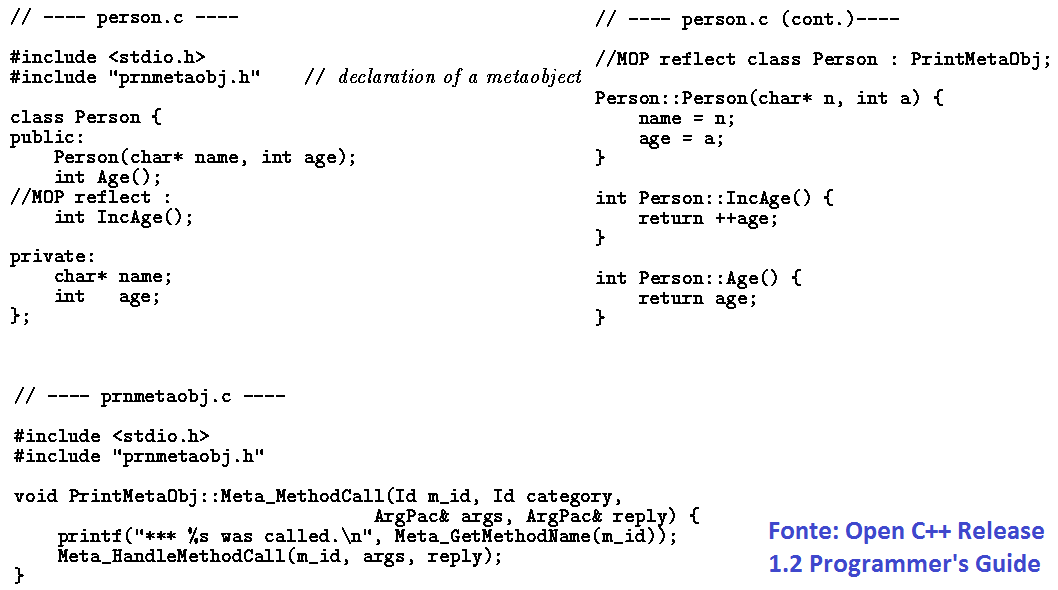
\includegraphics[width=1\textwidth]{example_open_cxx}
 	 	\end{block}
	 \end{frame}
	 \begin{frame}{Javaassist}
	 	Um pouco da história, e exemplos.
	 \end{frame}
	 \begin{frame}{Easymock}
	 	Mostrar o conceito de dynamic proxies do java (nativo)
	 	Mostrar como é implementado. 
	 	Fazer um paralelo com uma implementação em smalltalk, onde tem reflection ''de verdade'';
	 \end{frame}
 \section{Trabalhos Atuais}	 
 \begin{frame}{Trabalhos Atuais}
 	\alert{Escrever}
 \end{frame}
 \section{Referências}
 \begin{frame}[allowframebreaks]{Referências}
   \bibliography{apresentacao}
  \end{frame}
\end{document}

